\documentclass[10pt,a4paper]{article}

\usepackage[top=1.5cm, bottom=1.5cm, left=1.8cm, right=1.8cm]{geometry}
\usepackage{parskip}
\usepackage{titlesec}
\usepackage{enumitem}
\usepackage{multicol}
\usepackage{xcolor}
\usepackage{hyperref}
\usepackage[protrusion=false,expansion=false]{microtype}
\usepackage{tikz}
\usetikzlibrary{arrows.meta, positioning, backgrounds, fit}

% ── Colour palette ────────────────────────────────────────────────────────────
\definecolor{accent}  {RGB}{15,118,110}
\definecolor{cteal}   {RGB}{15,118,110}
\definecolor{cblue}   {RGB}{37, 99,235}
\definecolor{cpurple} {RGB}{124,58,237}
\definecolor{corange} {RGB}{194,65, 12}
\definecolor{cgreen}  {RGB}{5,150,105}
\definecolor{cgray}   {RGB}{75, 85, 99}

\hypersetup{colorlinks=true, urlcolor=accent, linkcolor=accent, pdfborder={0 0 0}}

% ── Section headings ─────────────────────────────────────────────────────────
\titleformat{\section}{\normalsize\bfseries\color{accent}}{}{0em}{}[\titlerule]
\titleformat{\subsection}{\small\bfseries}{}{0em}{}
\titlespacing{\section}   {0pt}{5pt}{2pt}
\titlespacing{\subsection}{0pt}{3pt}{1pt}

% ── List spacing ─────────────────────────────────────────────────────────────
\setlist[itemize] {noitemsep, topsep=1pt, leftmargin=1.2em}
\setlist[enumerate]{noitemsep, topsep=1pt, leftmargin=1.2em}
\setlength{\columnsep}{1.5em}
\setlength{\parskip}{2pt}

% ── TikZ node styles ─────────────────────────────────────────────────────────
\tikzset{
  bb/.style={rectangle, rounded corners=2pt,
             draw=#1!65!black, fill=#1!10,
             font=\tiny\bfseries, align=center,
             minimum height=0.48cm, inner xsep=4pt, inner ysep=2pt},
  arr/.style={-{Stealth[length=3.5pt,width=2.5pt]}, semithick, color=gray!55},
  lbl/.style={font=\tiny\itshape\color{gray!75}, midway},
}

% ── Helpers ───────────────────────────────────────────────────────────────────
\newcommand{\techfoot}{%
  \vspace{3pt}\rule{\linewidth}{0.4pt}\\
  {\footnotesize\color{gray!70}%
   \textbf{Stack:} Python\,3.13 · FastAPI · LangGraph (supervisor + HITL) ·
   LangChain · ChromaDB · FastMCP · Next.js\,16 · AWS Lambda · Bedrock · DynamoDB}%
}

% =============================================================================
\begin{document}

% ── Title ─────────────────────────────────────────────────────────────────────
\begin{center}
  {\large\bfseries Employee Onboarding AI Agent}\\[1.5pt]
  {\small\color{accent} Solution Design Document}
  \hspace{1em}{\footnotesize\color{gray!60}Acme Corp · August 2026}
\end{center}
\vspace{-2pt}\rule{\linewidth}{0.8pt}\vspace{3pt}

% =============================================================================
% DIAGRAM 1 — System Architecture (full width)
% =============================================================================
\begin{center}
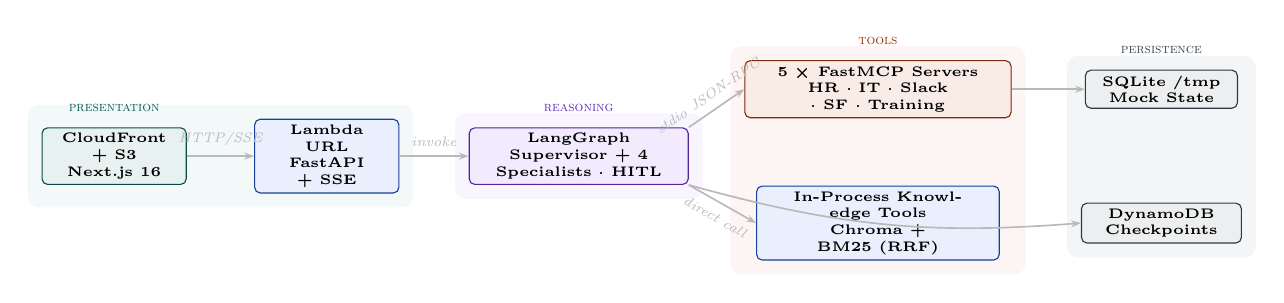
\begin{tikzpicture}
  % ── Nodes ──────────────────────────────────────────────────────────────────
  \node[bb=cteal,   text width=1.55cm] at (0,   0)    (fe)     {CloudFront + S3\\Next.js 16};
  \node[bb=cblue,   text width=1.55cm] at (2.7, 0)    (api)    {Lambda URL\\FastAPI + SSE};
  \node[bb=cpurple, text width=2.5cm]  at (5.9, 0)    (agent)  {LangGraph\\Supervisor + 4\\Specialists · HITL};
  \node[bb=corange, text width=3.1cm]  at (9.7, 0.85) (mcp)    {5 × FastMCP Servers\\HR · IT · Slack · SF · Training};
  \node[bb=cblue,   text width=2.8cm]  at (9.7,-0.85) (rag)    {In-Process Knowledge Tools\\Chroma + BM25 (RRF)};
  \node[bb=cgray,   text width=1.65cm] at (13.3, 0.85)(sqlite) {SQLite /tmp\\Mock State};
  \node[bb=cgray,   text width=1.75cm] at (13.3,-0.85)(chroma) {DynamoDB\\Checkpoints};

  % ── Arrows ─────────────────────────────────────────────────────────────────
  \draw[arr] (fe)    -- node[lbl, above] {HTTP/SSE}    (api);
  \draw[arr] (api)   -- node[lbl, above] {invoke}      (agent);
  \draw[arr] (agent.north east) -- node[lbl, above, sloped] {stdio JSON-RPC} (mcp.west);
  \draw[arr] (agent.south east) -- node[lbl, below, sloped] {direct call}    (rag.west);
  \draw[arr] (mcp)   -- (sqlite);
  \draw[arr] (agent.south east) to[bend right=10] (chroma.west);

  % ── Layer background bands ─────────────────────────────────────────────────
  \begin{scope}[on background layer]
    \node[rounded corners=4pt, fill=cteal!5, inner sep=5pt,
          fit=(fe)(api)] {};
    \node[rounded corners=4pt, fill=cpurple!5, inner sep=5pt,
          fit=(agent)] {};
    \node[rounded corners=4pt, fill=corange!5, inner sep=5pt,
          fit=(mcp)(rag)] {};
    \node[rounded corners=4pt, fill=cgray!6, inner sep=5pt,
          fit=(sqlite)(chroma)] {};
  \end{scope}

  % ── Layer labels ───────────────────────────────────────────────────────────
  \node[font=\tiny\color{cteal!80!black},   above=0.08cm of fe]     {\textsc{presentation}};
  \node[font=\tiny\color{cpurple!80!black}, above=0.08cm of agent]  {\textsc{reasoning}};
  \node[font=\tiny\color{corange!80!black}, above=0.08cm of mcp]    {\textsc{tools}};
  \node[font=\tiny\color{cgray!80!black},   above=0.08cm of sqlite] {\textsc{persistence}};
\end{tikzpicture}
\end{center}

\vspace{3pt}
% =============================================================================
% Two-column body
% =============================================================================
\begin{multicols}{2}

\section{Architecture}

The live site is a static Next.js export served from a private S3 bucket through CloudFront. The browser calls a public, response-streaming Lambda Function URL whose container runs FastAPI, LangGraph, and five MCP subprocesses. A LangGraph \textbf{supervisor} \texttt{StateGraph} routes each turn to one of four scoped \texttt{create\_react\_agent} specialist subgraphs; a hop cap of 3 prevents routing loops. Specialists dispatch over stdin/stdout JSON-RPC or call the in-process Chroma/BM25 knowledge tools. Mock SaaS state lives in SQLite under Lambda \texttt{/tmp}; durable conversation and interrupt checkpoints live in DynamoDB.

\section{AI Agent Application}

The supervisor is a pure router — it uses structured output (\texttt{Route\{next, reasoning\}}) to pick exactly one specialist per hop and never produces user-visible text. Each specialist owns a scoped toolbox, so tool choice stays tight (the Training Coach cannot accidentally file an IT ticket).

\begin{itemize}
  \item \textbf{HR Profile Specialist} — updates across HR Platform, Slack, and Salesforce; doubles as the onboarding planner for open-ended "what do I need to do?" questions.
  \item \textbf{Training Coach} — tracks four mandatory modules in order; never marks a module complete until the user explicitly says they finished it.
  \item \textbf{IT Access Specialist} — role-based recommendations → user picks → manager approval → IT ticket; each write is gated.
  \item \textbf{Knowledge Expert} — hybrid-RAG Q\&A over seven policy documents with source attribution; read-only.
\end{itemize}

Specialists are written as collaborators: they ask one focused question when information is missing, propose changes before writing, and narrate progress briefly. Direct imperatives with full values execute immediately — the HITL gate is the final review, not a substitute for conversation.

Amazon Bedrock Nova is the AWS chat provider and Titan Text Embeddings v2 builds the RAG index. Local development keeps the OpenAI/Ollama provider path.

\subsection{RAG Pipeline (3 production techniques)}
\begin{enumerate}
  \item \textbf{Cosine similarity} — ChromaDB collection configured with \texttt{hnsw:space=cosine} so relevance is magnitude-independent.
  \item \textbf{Contextual chunking} — each chunk is prefixed with its document title and section header before embedding, preserving meaning in isolation.
  \item \textbf{Hybrid retrieval} — BM25 keyword search and vector semantic search merged via Reciprocal Rank Fusion (equal 0.5/0.5 weighting with \texttt{EnsembleRetriever}).
\end{enumerate}

\section{Human-in-the-Loop}

Eight destructive tools (every \texttt{update\_*}, \texttt{add\_to\_slack\_channels}, \texttt{assign\_salesforce\_permission\_set}, \texttt{complete\_training\_module}, \texttt{request\_manager\_approval}, \texttt{submit\_it\_ticket}) are wrapped at load time with a LangGraph \texttt{interrupt()} gate. When a specialist calls one, the graph pauses, the API emits an \texttt{approval\_required} SSE event, and the frontend renders an inline approval card where the user can review arguments, \textbf{edit any string field}, then approve or reject. Only changed keys are sent as \texttt{edited\_args}; the wrapper merges them (\texttt{\{**kwargs, **edited\_args\}}) before invoking the underlying tool. State is checkpointed by DynamoDB on AWS or \texttt{MemorySaver} locally, so the approval survives across separate HTTP turns; rejections are fed back as a \texttt{[SKIPPED]} tool message the specialist handles gracefully.

\section{Evaluation}

A golden-dataset harness (\texttt{python -m evals.run\_evals}) exercises the full supervisor graph across 15 cases — HR, Training, IT, Knowledge, and routing edges. Each case runs on a fresh \texttt{thread\_id} (so cases cannot leak state) and is graded by four deterministic hard-gate evaluators — \textit{routing}, \textit{tool\_trajectory}, \textit{tool\_choice}, \textit{response\_contains} — plus an LLM-as-judge scoring response quality (1–5) against a per-case rubric. The runner exits non-zero on any hard-gate failure, so it drops straight into CI; runs are traced to LangSmith when tracing is enabled.

\section{Orchestration}

\textbf{Request flow:} \texttt{POST /api/chat} → FastAPI invokes the orchestrator → supervisor routes to a specialist → specialist issues tool calls (possibly pausing at an HITL gate) → results stream back as SSE (\texttt{agent\_handoff}, \texttt{tool\_call}, \texttt{tool\_result}, \texttt{approval\_required}, \texttt{text\_delta}, \texttt{done}). Interrupted runs resume via \texttt{POST /api/chat/resume} with the approval decision.

\textbf{MCP communication:} Each of the five servers is a subprocess spawned at startup. \texttt{langchain-mcp-adapters} serialises tool calls to JSON-RPC over stdin/stdout; the HITL wrapper sits between the adapter and the specialist so gating is transparent to both sides.

\textbf{Memory:} \texttt{DynamoDBSaver} on AWS (or \texttt{MemorySaver} locally) keeps per-employee conversation history \textit{and} graph interrupt state keyed by \texttt{thread\_id}, so multi-turn context and paused approvals survive between HTTP requests and, on AWS, Lambda recycling.

\section{AWS Deployment}

Terraform provisions CloudFront, a private S3 frontend origin, a public Lambda Function URL, ECR, DynamoDB checkpoints, CloudWatch logs, and an EventBridge warmer. GitHub Actions assumes an IAM role through OIDC only from the public repository's \texttt{main} branch and allowed environments. Deployments tag the backend image with the commit SHA, apply Terraform, bake the emitted API URL into the frontend, synchronize S3, invalidate CloudFront, and smoke-test health plus all 20 tools. Live site: \href{https://d2j7378c90nw96.cloudfront.net}{d2j7378c90nw96.cloudfront.net}.

\section{Trade-offs \& Considerations}

\subsection{Assumptions \& Trade-offs}
\begin{itemize}
  \item \textbf{In-process RAG} — ChromaDB's embedded SQLite is unsafe for cross-process access. Knowledge tools run in the main process, sacrificing isolation to avoid file-lock deadlocks.
  \item \textbf{Ephemeral mock data} — Lambda stores SQLite, Chroma, and BM25 under \texttt{/tmp}. New or concurrent execution environments can reset or diverge; only DynamoDB graph checkpoints are durable.
  \item \textbf{Mock MCP servers} — simulate Workday, ServiceNow, Slack, Salesforce, and an LMS. Production integration needs OAuth, rate limiting, and idempotency guards.
  \item \textbf{Public demo} — the Function URL has no AWS authentication. CORS restricts browsers but does not authenticate callers.
\end{itemize}

\subsection{Scalability}
The DynamoDB checkpointer supports Lambda process churn, but the mock SQLite systems do not provide shared horizontal state. The BM25 index rebuilds at startup — fine for a static knowledge corpus; a dynamic knowledge base needs incremental indexing and a managed vector store. Real SaaS integrations should replace the embedded mock database.

\subsection{Security \& Governance}
\begin{itemize}
  \item \texttt{employee\_id} selects mock data; it is not identity or authorization.
  \item Sensitive fields (salary, SSN) should be excluded via field-level access control before reaching LLM context.
  \item CloudWatch receives structured logs; production audit events should be shipped to a SIEM with PII controls.
  \item The API and \texttt{/api/admin/reset-db} require authentication, RBAC, and rate limiting before real data is used.
  \item Reserved concurrency is disabled for the current account quota, so it is not a spend cap. Add Budgets/alarms and throttling; Bedrock, Lambda, the warmer, logs, ECR, DynamoDB, S3, and CloudFront can incur charges.
\end{itemize}

\end{multicols}

% =============================================================================
% DIAGRAM 2 — Multi-Agent Topology (full width)
% =============================================================================
\vspace{2pt}
\noindent{\normalsize\bfseries\color{accent}Supervisor Graph · HITL · Evals}
\vspace{2pt}
\rule{\linewidth}{0.5pt}
\vspace{3pt}

\begin{center}
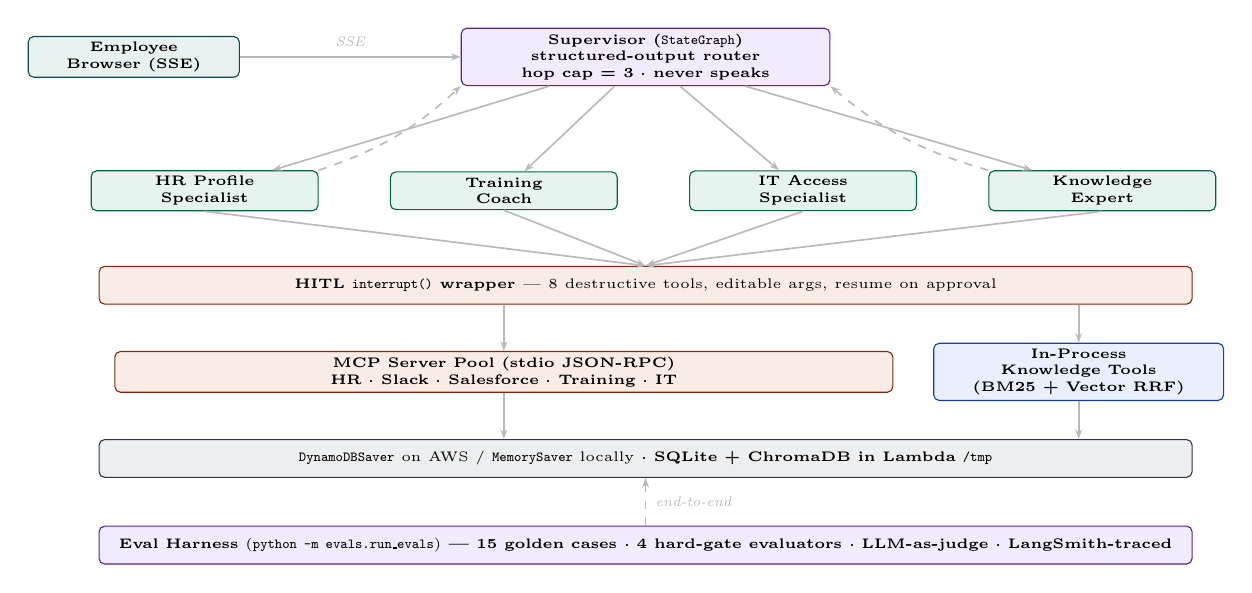
\begin{tikzpicture}
  % ── User + Supervisor ──────────────────────────────────────────────────────
  \node[bb=cteal,   text width=2.4cm] at (0.5, 3.8) (user)
      {Employee\\Browser (SSE)};
  \node[bb=cpurple, text width=4.4cm] at (7.0, 3.8) (sup)
      {\textbf{Supervisor} (\texttt{StateGraph})\\structured-output router\\hop cap = 3 · never speaks};

  % ── Specialist agents ──────────────────────────────────────────────────────
  \node[bb=cgreen, text width=2.6cm] at (1.4, 2.1) (hrp)
      {HR Profile\\Specialist};
  \node[bb=cgreen, text width=2.6cm] at (5.2, 2.1) (trc)
      {Training\\Coach};
  \node[bb=cgreen, text width=2.6cm] at (9.0, 2.1) (ita)
      {IT Access\\Specialist};
  \node[bb=cgreen, text width=2.6cm] at (12.8,2.1) (knw)
      {Knowledge\\Expert};

  % ── HITL band ──────────────────────────────────────────────────────────────
  \node[bb=corange, text width=13.6cm] at (7.0, 0.9) (hitl)
      {\textbf{HITL \texttt{interrupt()} wrapper}
       \textmd{— 8 destructive tools, editable args, resume on approval}};

  % ── Tool pool ──────────────────────────────────────────────────────────────
  \node[bb=corange, text width=9.6cm] at (5.2,-0.2) (pool)
      {MCP Server Pool (stdio JSON-RPC)\\
       HR · Slack · Salesforce · Training · IT};
  \node[bb=cblue, text width=3.4cm] at (12.5,-0.2) (rag)
      {In-Process\\Knowledge Tools\\(BM25 + Vector RRF)};

  % ── Shared state ───────────────────────────────────────────────────────────
  \node[bb=cgray, text width=13.6cm] at (7.0,-1.3) (shared)
      {\texttt{DynamoDBSaver} \textmd{on AWS / \texttt{MemorySaver} locally}
       · SQLite + ChromaDB in Lambda \texttt{/tmp}};

  % ── Eval harness ───────────────────────────────────────────────────────────
  \node[bb=cpurple, text width=13.6cm] at (7.0,-2.4) (evals)
      {\textbf{Eval Harness} \textmd{(\texttt{python -m evals.run\_evals})}
       — 15 golden cases · 4 hard-gate evaluators · LLM-as-judge · LangSmith-traced};

  % ── Arrows ─────────────────────────────────────────────────────────────────
  \draw[arr] (user) -- node[lbl, above] {SSE} (sup);
  \draw[arr] (sup) -- (hrp);
  \draw[arr] (sup) -- (trc);
  \draw[arr] (sup) -- (ita);
  \draw[arr] (sup) -- (knw);
  \draw[arr, dashed] (hrp.north east) to[bend right=12] (sup.south west);
  \draw[arr, dashed] (knw.north west) to[bend left=12]  (sup.south east);
  \draw[arr] (hrp.south) -- (hitl.north);
  \draw[arr] (trc.south) -- (hitl.north);
  \draw[arr] (ita.south) -- (hitl.north);
  \draw[arr] (knw.south) -- (hitl.north);
  \draw[arr] (hitl.south -| pool.north) -- (pool.north);
  \draw[arr] (hitl.south -| rag.north)  -- (rag.north);
  \draw[arr] (pool.south) -- (shared.north -| pool.south);
  \draw[arr] (rag.south)  -- (shared.north -| rag.south);
  \draw[arr, dashed] (evals.north) -- node[lbl, right] {end-to-end} (shared.south);
\end{tikzpicture}
\end{center}

\noindent{\footnotesize The supervisor is a pure router; each specialist is a \texttt{create\_react\_agent} subgraph with a \textit{scoped} toolbox, so tool choice stays tight by construction. Eight destructive tools pass through an \texttt{interrupt()} wrapper that surfaces an editable approval card before a write; DynamoDB checkpoints the paused graph on AWS. The public demo runs behind CloudFront with a response-streaming Lambda backend, Bedrock models, and Terraform/GitHub Actions delivery. A 15-case golden dataset gates CI on routing, tool-trajectory, tool-choice, and response-contains failures.}

\vspace{4pt}
\techfoot

\end{document}
